\documentclass[a4paper, 12pt]{article}
% page
% \usepackage[top=2.54cm,bottom=2.54cm,left=3.18cm,right=3.18cm]{geometry}  % default
\usepackage{graphicx}
\usepackage[top=2.27cm,bottom=1.27cm,left=1.27cm,right=1.27cm]{geometry}
% \usepackage[none]{hyphenat} % remove hyphen
\usepackage[hidelinks]{hyperref}    % remove hyperref box

% header and footer
\usepackage{fancyhdr}
\fancypagestyle{plain}{
    \fancyhead[L]{}
    \fancyhead[C]{Computer Vision HW4 Report}
    \fancyhead[R]{Student ID: R11625015\\ Name: 廖致豪}
    % \fancyfoot[L]{}
    % \fancyfoot[C]{}
    % \fancyfoot[R]{}
    \renewcommand{\headrulewidth}{0.5pt}
    \renewcommand{\footrulewidth}{0pt}
    % \setlength{\headheight}{}
    % \addtolength{\topmargin}{}
}
\pagestyle{plain}

% font setting
\usepackage{fontspec}
\usepackage{xeCJK}
    \setCJKmainfont{標楷體}
    % \setCJKmainfont{微軟正黑體}
    \XeTeXlinebreaklocale "zh"
    \XeTeXlinebreakskip = 0pt plus 1pt
    \defaultCJKfontfeatures{AutoFakeBold=true,AutoFakeSlant=true}
    % \newCJKfontfamily\Kai{標楷體}
    \newCJKfontfamily\Hei{微軟正黑體}
    \newCJKfontfamily\NewMing{新細明體}
    \setmainfont{Arial}   % Set English to Arial

% codestyle
\usepackage{listings}
\usepackage{xcolor}
\definecolor{codegreen}{rgb}{0,0.6,0}
\definecolor{codegray}{rgb}{0.5,0.5,0.5}
\definecolor{codepurple}{rgb}{0.58,0,0.82}
\definecolor{backcolour}{rgb}{0.95,0.95,0.92}

\lstdefinestyle{mystyle}{
    backgroundcolor=\color{backcolour},   
    commentstyle=\color{codegreen},
    keywordstyle=\color{magenta},
    numberstyle=\tiny\color{codegray},
    stringstyle=\color{codepurple},
    basicstyle=\ttfamily\footnotesize,
    breakatwhitespace=false,         
    breaklines=true,                 
    captionpos=b,                    
    keepspaces=true,                 
    numbers=left,                    
    numbersep=5pt,                  
    showspaces=false,                
    showstringspaces=false,
    showtabs=false,                  
    tabsize=2
}

\lstset{style=mystyle}

% packages
\usepackage{tabularx, array, slashbox}
\usepackage{makecell}
\usepackage{multirow}
\usepackage{float}
\usepackage{amsmath}
\usepackage{url}
\usepackage{subcaption}
\usepackage{tikz}
\usepackage{mathtools}
% \usepackage{indentfirst}

% main page
\begin{document}
\section{Visualize the disparity map of 4 testing images.}
\begin{table}[!htb]
    \centering
    \caption{Disparity map visualization of four testing images}
    \begin{tabular}{|c|c|}
        \hline
        Tsukuba                                    & Venus                                    \\
        \hline
        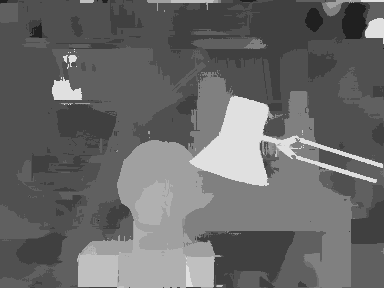
\includegraphics[scale=0.5]{./Tsukuba.png} & 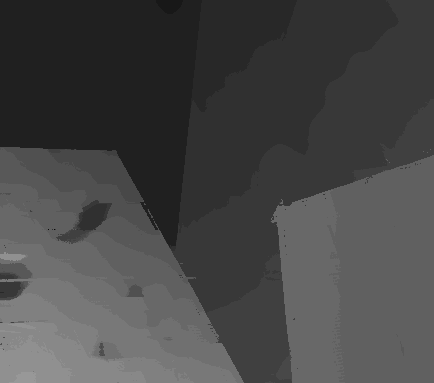
\includegraphics[scale=0.5]{./Venus.png} \\
        \hline
        Teddy                                      & Cones                                    \\
        \hline
        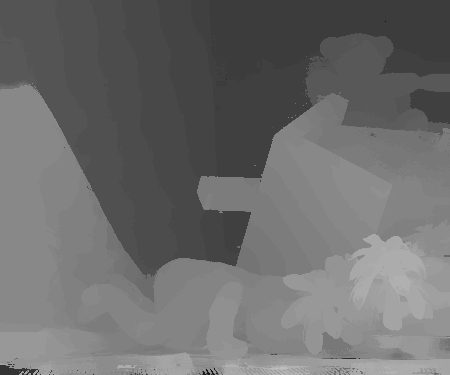
\includegraphics[scale=0.5]{./Teddy.png}   & 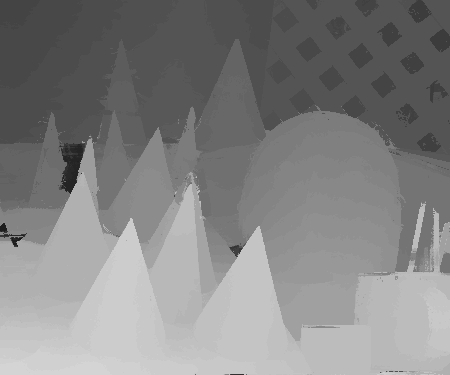
\includegraphics[scale=0.5]{./Cones.png} \\
        \hline
    \end{tabular}
\end{table}

\section{Report the bad pixel ratio of 2 testing images with given ground truth (Tsukuba/Teddy).}

\begin{table}[!htb]
    \centering
    \caption{Bad pixel ratio analysis for two test images (Tsukuba/Teddy)}
    \begin{tabular}{|c|c|c|c|c|c|}
        \hline
                & bad pixel ratio \\
        \hline
        Tsukuba & 4.44\%          \\
        \hline
        Teddy   & 9.48\%          \\
        \hline
    \end{tabular}
\end{table}

\section{Describe your algorithm in terms of 4-step pipeline.}
The algorithm in computeDisp function can be described in terms of a 4-step pipeline:

1. Cost computation

In the first step, the algorithm computes the matching cost between the left image (Il) and the right image (Ir). It uses the concept of Census cost, which involves converting 8-neighbor pixel values into local binary patterns and then calculating the Hamming distance between corresponding pixels in the two images. The algorithm also computes the cost both from Il to Ir and from Ir to Il for later left-right consistency.

2. Cost aggregation

In order to calculate the cost aggregation, the algorithm refines the computed cost by considering nearby costs. Since joint bilateral filter takes into account both the intensity similarity and spatial proximity of pixels to preserver edges whlie smoothing the cost, it is used in the algorighm to filter the cost volume for each disparity value.

3. Disparity optimization

In this step, the algorithm determines the disparity (depth) based on the estimated cost. It uses a winner-take-all approach, where it selects the disparity with the minimum cost for each pixel location. This results in a disparity map for both the left and right images.

4. Disparity refinement

In this final step, the algorithm enhances the disparity map by performing various refinements. It starts with a left-right consistency check, where it compares the disparities from the left and right images to ensure consistency, followed by performing hole filling to fill in any missing or invalid disparity values. Finally, it applies weighted median filtering to further refine the disparity map, taking into account the intensity values of the pixels.

Overall, this 4-step pipeline allows the algorithm to compute high accurate and refined disparity map from a pair of stereo images.

% BibTex
% \bibliographystyle{ieeetr}
% \bibliography{reference}

\end{document}